%qqqqqqqqqqqqqqqqqqqqqqqqqqqqqqqqqqqqqqqqqqqqqqqqqqqqqqqqqqqqqqqqqqqqqqqqq
%Quote
\begin{savequote}[50mm]
‘‘Todos los efectos de la Naturaleza son sólo la consecuencia matemática 
de un pequeño número de leyes inmutables’’
\qauthor{Pierre Simon Laplace}
\end{savequote}
%qqqqqqqqqqqqqqqqqqqqqqqqqqqqqqqqqqqqqqqqqqqqqqqqqqqqqqqqqqqqqqqqqqqqqqqqq




%#########################################################################
\chapter{Métodos Computacionales en Cosmología}
\label{cha:N-BodySimulations}


En los últimos años la física computacional ha adquirido un papel 
importante en física, permitiendo modelar diversos sistemas complejos sin
necesidad de recurrir a la experimentación u observación. Entre los 
métodos abarcados por la física computacional destaca el problema de 
N-cuerpos debido a que muchos fenómenos requieren el cómputo de 
interacciones entre una gran cantidad de cuerpos. Algunos ejemplos muy 
representativos son la modelación de sistemas moleculares, física de 
plasmas y especialmente problemas gravitacionales en astrofísica. El 
desarrollo de los métodos específicos para la solución de este tipo de 
problemas antecede la aparición de los ordenadores y sistemas de cómputo 
en general, aún así, el desarrollo de estos potenció enormemente esta área
al punto de ser la física computacional una nueva rama de la física.


En este capítulo se desarrollan métodos específicos para la solución de 
proble\-mas gravitacionales en astrofísica, en especial para la simulación
del universo a gran escala en régimen no lineal, partiendo de algoritmos 
básicos para el cómputo de fuerzas, métodos de detección de halos, hasta 
esquemas de clasificación para el entorno cosmológico.
 

%#########################################################################




%*************************************************************************
%N-body Simulations
\section{Simulaciones de N-Cuerpos}
\label{sec:N-bodySimulations}


En general, el tipo de fenómenos más promisorios para ser modelados con 
simulaciones N-cuerpos son aquellos donde las interacciones son 
fuertemente ligadas entre las partículas, tales como fuerzas de largo 
alcance o correlaciones no locales. En la figura \ref{fig:NbodyProblem}
se ilustra un conjunto de partículas puntuales que interactúan mutuamente 
bajo alguna campo de fuerza $\bds f$, estas condiciones conforman la 
formulación clásica del problema de N-cuerpo.

\
%.........................................................................
%N-Body Problem
\begin{figure}[htbp]
	\centering
	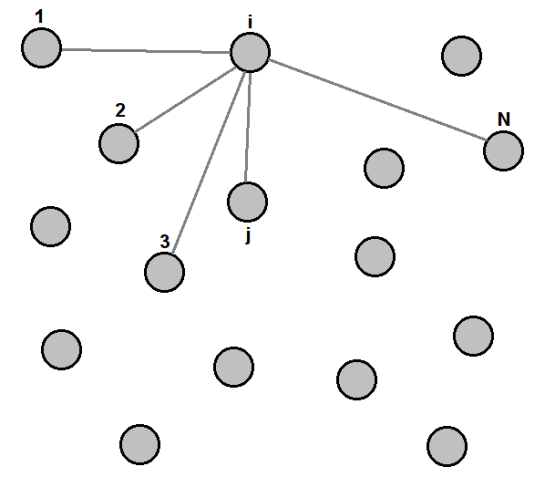
\includegraphics[width=0.50\textwidth]
	{./figures/3_nbody_simulations/Nbody_Problem.png}

	\caption{\small{Formulación del problema de N-cuerpos.}}
	
	\label{fig:NbodyProblem}
\end{figure}
%.........................................................................


Asumiendo interacciones que dependen de la posición\footnote{En el 
problema generalizado las interacciones pueden depender de otros 
parámetros tales como velocidad o grados de libertan intrínsecos como 
espín.}, la ecuación de movimiento para la partícula $i$ de la figura
\ref{fig:NbodyProblem} queda \cite{pfalzner1996} \cite{binney2008}


%.........................................................................
%Movement Equation
\eq{eq:MovementEquation}
{ \ddot{ \bds r}_i = \sum_{j=1}^N \bds f( \bds r_i, \bds r_j ) = -\nabla 
\phi( \bds r_i )\ \ \ \ \ \ \ i=1,2,\cdots,N }
%.........................................................................
donde se ha introducido la función potencial $\Phi(\bds r)$. Para el caso 
de interacción gravitacional el potencia adquiere la forma


%.........................................................................
%Gravitational Potential
\eq{eq:GravitationalPotential}
{ \phi(\bds r) = -\sum_{j=1}^N  \frac{G m_j}{|\bds r - \bds r_j|} }
%.........................................................................


La solución se obtiene a partir del conjunto $\{ \bds r_1(t),\cdots, 
\bds r_N(t) \}$ determinado a partir de las ecuaciones 
\ref{eq:MovementEquation}, para lo cual es necesario implementar 
aproximaciones numéricas debido a la no solubilidad analítica del 
problema.


	%---------------------------------------------------------------------
	%Direct sum
	\subsection{Método P-P}
	\label{subsec:PPMethos}
	%---------------------------------------------------------------------
	
	
La primera aproximación para la solución de las ecuaciones de movimiento
\ref{eq:MovementEquation} es computar todas las $N-1$ interacciones de la 
$i$-ésima partícula con todas las demás en un cierto tiempo $t$ y esto 
para $i=1,2,\cdots N$, luego a partir de un esquema numérico de 
integración se calculan las posiciones en un tiempo posterior discretizado
$t+\Delta t$ y así hasta un tiempo máximo $t_{\submath{max}}$ deseado. 
Este método se denomina P-P (Partícula a Partícula) y es uno de los tres 
métodos estándar desa\-rrollados para la solución del problema de 
N-cuerpos.


Cuando las interacciones poseen singularidades, tal como los potenciales
Cou\-lombianos de la electrostática y la gravitación (ecuación 
\ref{eq:GravitationalPotential}), la integración de las ecuaciones de 
movimiento se hace sensible a encuentro cercanos entre partículas y por 
tanto debe aumentarse la resolución en la discretización temporal, 
llevando a un aumento considerable en el tiempo de cómputo. Una solución 
común es introducir un parámetro de suavizado que elimine estas 
singularidades, aunque a costa de una pérdida en la precisión de la 
solución. Para el potencial gravitacional \ref{eq:GravitationalPotential} 
queda


%.........................................................................
%Gravitational Potential
\eq{eq:SoftPotential}
{ \phi_{s}(\bds r) = -\sum_{j=1}^N  \frac{G m_j}{|\bds r - \bds r_j| 
+ \epsilon_j^2} }
%.........................................................................
donde $\epsilon_j$ es el parámetro de suavizado y puede interpretarse como 
una medida de la dimensión física real de la partícula.


A pesar de la alta precisión lograda con este método, el tiempo de cómputo
escala como $t_{\submath{comp}}\propto N^2$, lo que lo hace altamente 
inviable para un gran número de partículas (generalmente 
$N\gtrsim 10^4-10^5$ \cite{padmanabhan1995}). Para la simulación de 
sistemas planetarios, órbitas de cuerpos menores y cúmulos estelares este 
método resulta ser muy adecuado, pero para problemas cosmológicos y de 
galaxias, donde el número de partículas debe ser el máximo posible para 
poder reproducir la verdadera naturaleza continua de las distribuciones de 
materia, es necesario desarrollar métodos menos costosos 
computacionalmente.


	%---------------------------------------------------------------------
	%Tree codes
	\subsection{Método PM}
	\label{subsec:PMMethod}
	%---------------------------------------------------------------------
	
	
Un segundo esquema para el cómputo del problema de N-cuerpos es el método 
PM\footnote{PM viene de la siglas en inglés \textit{Particle Mesh} y 
una traducción adecuada sería malla de partículas.}\cite{dawson1983}, este 
consiste en determinar una distribución continua del campo de densidad a 
partir de las masas y posiciones de las partículas, para esto se divide el 
espacio de la simulación en una malla de $M\times M\times M$ celdas y se 
hace un conteo del número de partículas por celda para asociar un valor 
específico de masa y por tanto de densidad. Un esquema ilustrativo es 
mostrado en la figura \ref{fig:MP_Method}


%.........................................................................
%PM Method
\begin{figure}[htbp]
	\centering
	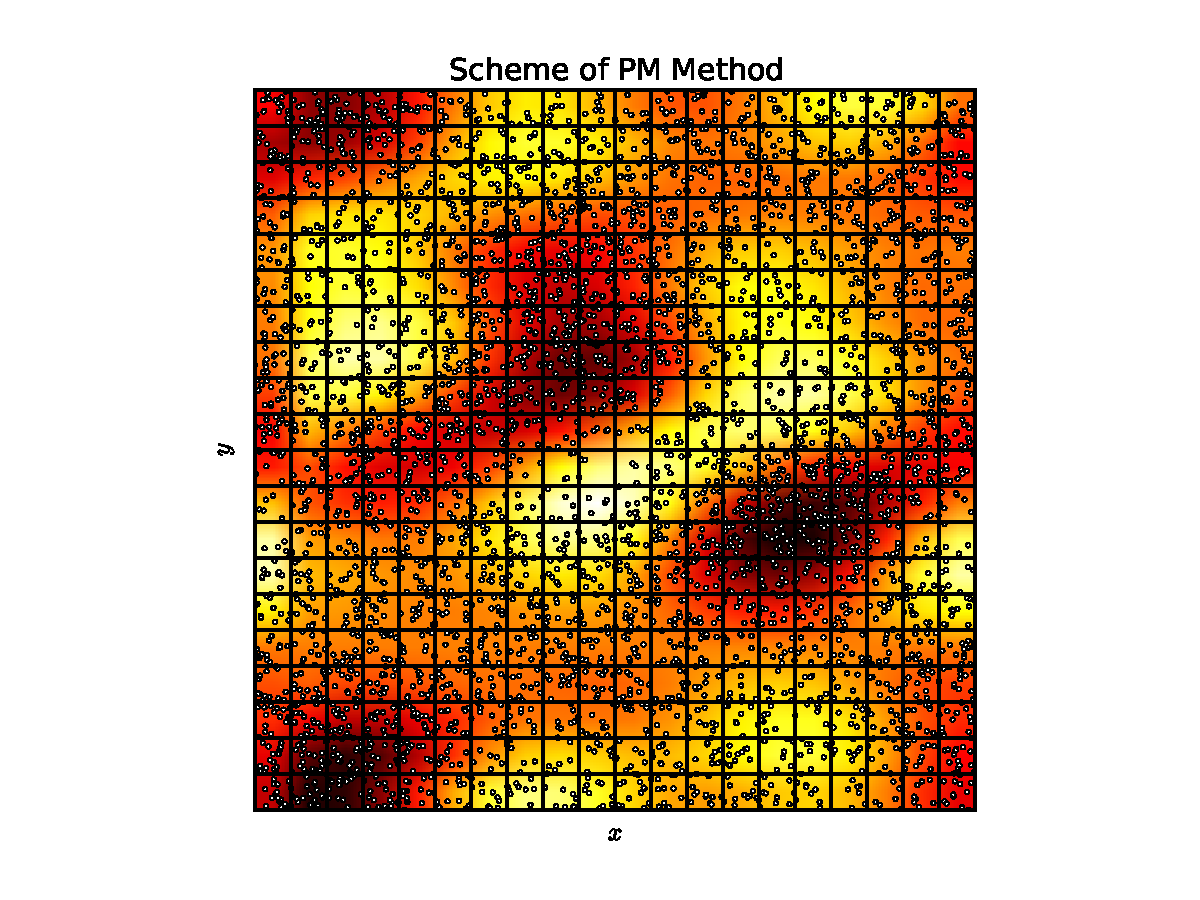
\includegraphics[width=1.00\textwidth]
	{./figures/3_nbody_simulations/PM_Method.pdf}

	\caption{\small{Diagrama ilustrativo del método P$^3$M. El mapa 
	dibujado sobre la distribución de partículas corresponde a la densidad
	asociada a cada celda de la malla. Las zonas oscuras corresponden a 
	regiones de sobredensidad mientras las zonas blancas a regiones de 
	menor densidad, acorde a la cantidad de partículas por celda y sus 
	masas individuales.}}
	
	\label{fig:MP_Method}
\end{figure}
%.........................................................................

\newpage
El método puede ser resumido en los siguientes pasos


%.........................................................................
%Particle Mesh steps
\begin{itemize}
\item[\textbf{1.}] A partir de la malla establecida sobre la simulación es
calculado un campo de densidad continuo $\rho(\bds r)$ interpolado entre 
cada celda.

\item[\textbf{2.}] Con el campo de densidad se procede a computar el 
potencial en la ecuación de movimiento \ref{eq:MovementEquation} a través 
de la ecuación de Poisson


%.........................................................................
%Poisson Equation
\eq{eq:Poisson}
{ \nabla^2 \phi = 4 \pi G \rho }
%.........................................................................


Para esto generalmente son usados esquemas de integración basados en la
transformada de Fourier, tales como la transformada rápida de Fourier 
(FFT por su siglas en inglés).

\item[\textbf{3.}] Usando el campo de potencial anterior se calcula la 
posición de cada partícula en el tiempo siguiente $t+\Delta t$, y se 
repite el esquema completo hasta un tiempo máximo deseado.

\end{itemize}
%.........................................................................


Este método es menos preciso que el método de suma directa, aún así es 
posible demostrar que el tiempo de cómputo escala como $t_{\submath{comp}} 
\propto N + M \log M$, con un comportamiento asintótico de 
$t_{\submath{comp}} \propto N$ para altas resoluciones $M$ de la malla y 
$t_{\submath{comp}} \propto N$ para bajas resoluciones \cite{pfalzner1996}.
En todos los casos la eficiencia es mucho mayor que el método PM 
\ref{subsec:PMMethod} cuando el número de partículas es relativamente 
grande $N\ll 10^4 - 10^5$, lo que hace a este método bastante competente 
para problemas de muchas partículas.


Existen algunas situaciones patológicas para las cuales el método presenta
dificultades \cite{pfalzner1996}


%.........................................................................
%Difficulties of PM Method
\begin{itemize}
\item Distribuciones de partículas altamente inhomogéneas.
\item Sistemas fuertemente correlacionados.
\item Sistemas con geometrías no triviales.
\end{itemize}
%.........................................................................


Debido a las altas inhomogeneidades y fuertes correlaciones locales por 
acople gravitacional entre de los diferentes modos en el universo tardío 
($z\gtrsim 8$), este método resulta poco preciso para la simulación del 
régimen no lineal. 


	%---------------------------------------------------------------------
	%Hidrodynamical and dark matter simulations
	\subsection{Método P$^3$M}
	\label{subsec:P3Method}
	%---------------------------------------------------------------------
	
	
El último los tres esquemas estándar para simulaciones de N-Cuerpos es el 
método P$^3$M (PP $+$ PM) \cite{hockney1988}, este es una combinación de 
los métodos anteriores, haciendo uso de las ventajas de cada uno.


%.........................................................................
%P3M Method
\begin{figure}[htbp]
	\centering
	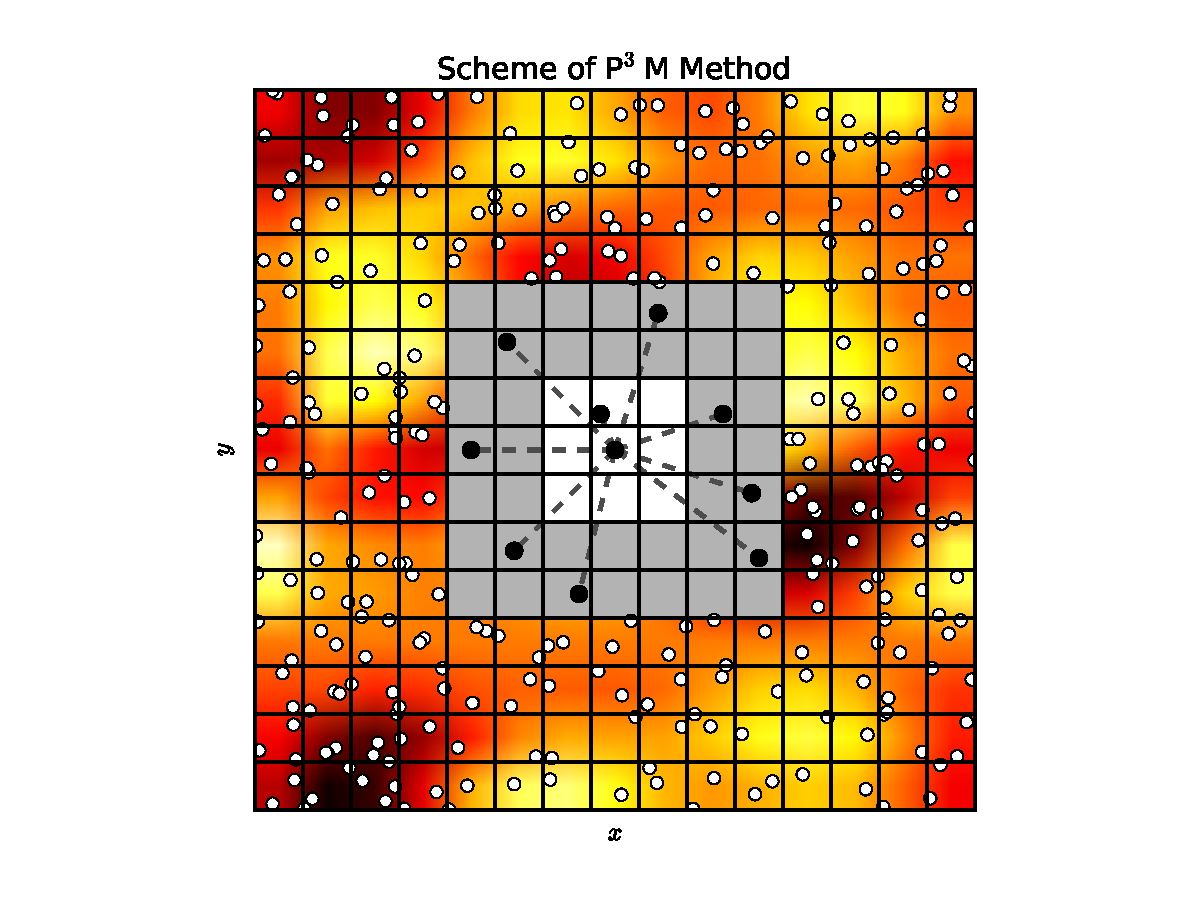
\includegraphics[width=1.00\textwidth]
	{./figures/3_nbody_simulations/P3M_Method.pdf}

	\caption{\small{Diagrama ilustrativo del método P$^3$M. Para la 
	partícula de referencia en el centro la interacción con partículas 
	lejanas es calculada con el método PM, mientras que para las 
	partículas cercanas en la región gris y blanca es usado el método de 
	suma directa PP.}}
	
	\label{fig:P3M_Method}
\end{figure}
%.........................................................................


En la figura \ref{fig:P3M_Method} se ilustra el método P$^3$M, en cada
paso de integración del sistema se hace un grid jerárquico respecto a cada
partícula, las jerarquías son definidas de acuerdo a la distancias 
relativas y determinan la aproximación usada para el cómputo de la 
ecuación de movimiento. Para partículas cercanas (primera jerarquía) se 
usa el método de suma directa, lo que permite dar cuenta de correlaciones
locales y dar un tratamiento adecuado a zonas con altas inhomogeneidades.
En las siguientes jerarquías se descompone el potencial en sus componentes
multipolares, tomando las contribuciones de más alto orden acorde al nivel 
de la jerarquía, así por ejemplo la segunda jerarquía tiene en cuenta las 
contribuciones dipolares, la tercera las cuadrupolares, etc. Finalmente 
para la última jerarquía se usa el esquema PM, interpolando el campo de 
densidad y resolviendo la ecuación de Poisson \ref{eq:Poisson} para el 
potencial.


%.........................................................................
%Tree Code Building
\begin{figure}[htbp]
	\centering
	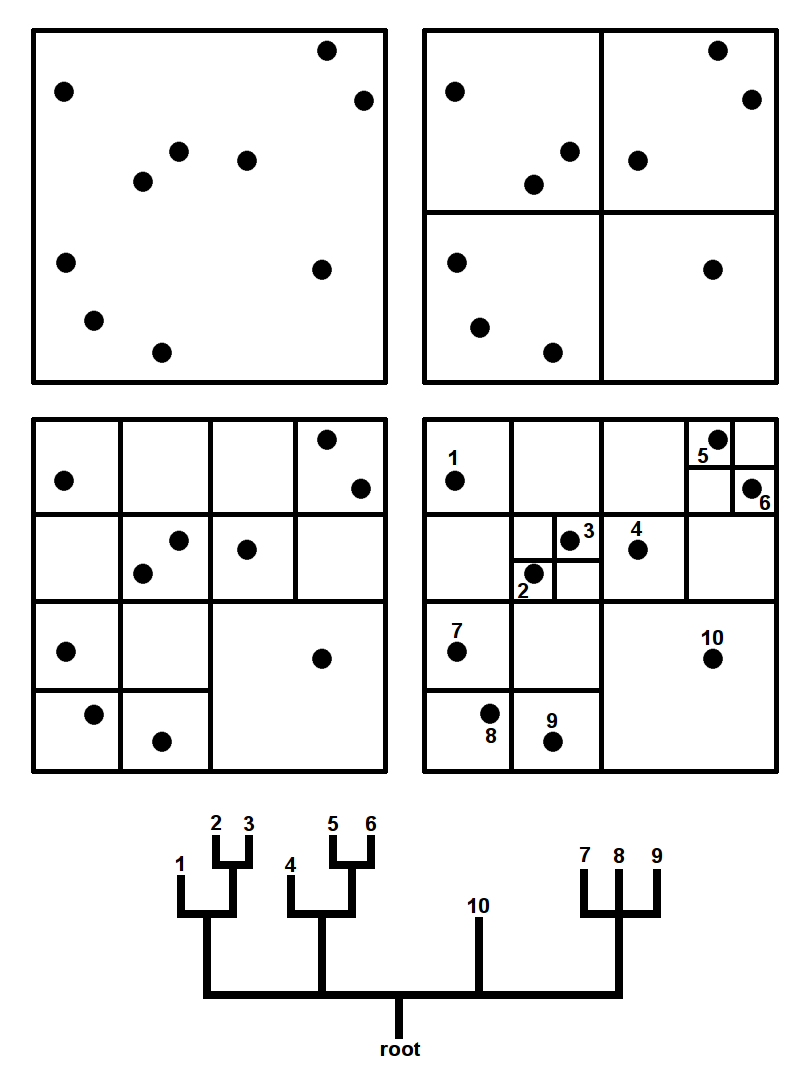
\includegraphics[width=0.72\textwidth]
	{./figures/3_nbody_simulations/TreeCode.png}

	\caption{\small{Ejemplo de construcción de un código de árbol para
	una simulación de N-cuerpos. En los paneles superiores se muestran
	iteraciones del método para un problema 2D. En la parte inferior se
	ilustra el árbol construido con cada partícula de la simulación.}}
	
	\label{fig:Tree_Code}
\end{figure}
%.........................................................................
\newpage

Uno de los principales inconvenientes de este método radica en la 
construcción de la estructura jerárquica para la evaluación de las 
interacciones. El esquema original propuesto simultáneamente por 
\cite{appel1985} \cite{jernigan1985} y \cite{porter1985} presenta
inconsistencias debido a la falta de fundamentación física en la 
construcción de la estructura jerárquica \cite{pfalzner1996}.


Uno de los métodos propuestos para la construcción de la estructura 
jerárquica y que carece en gran medida de las inconsistencias mencionados 
se denomina código de árbol octante y fue inicialmente desarrollado por 
\cite{barnes1986}. En este algorítmo el espacio de la simulación es 
embebido en una celda cúbica denominada raíz (\textit{root}) y luego se 
divide en 8 regiones de igual tamaño denominadas octantes, estas componen 
la primera jerarquía del árbol. El método se repite de forma recursiva 
hasta obtener a lo sumo una partícula por celda, construyendo de esta 
forma un conjunto de jerarquías que determinan las vecindades de todas las 
partículas. En la figura \ref{fig:Tree_Code} se ilustra las iteraciones 
requeridas para la construcción del árbol en una simulación (por 
simplicidad se ha tomado en dos dimensiones) y en la parte inferior de la 
misma figura se muestra esquemáticamente la estructura del árbol. De esta 
forma es posible computar por ejemplo la interacción entre las partículas 
7, 8 y 9 con suma directa, por ser vecinas próximas, mientras que su 
interacción con las demás partículas, pertenecientes a otras ramas, por 
medio de PM.


%*************************************************************************




%*************************************************************************
%Types of simulations
\section{Tipos de Simulación}
\label{sec:Types of Simulations}


Usando los métodos descritos en la anterior subsección es posible realizar
simulaciones del universo en régimen no lineal y estudiar su comportamiento 
de forma numérica. Debido a que en régimen no lineal los procesos 
astrofísicos de grandes escalas son dominados principalmente por materia 
oscura, es habitual no consi\-derar la contribución de las componentes de 
radiación y materia bariónica, además de que los procesos físicos que 
involucran estás componentes aumentarían conside\-rablemente los tiempos 
de cómputo. Este tipo de simulaciones son denominadas \textit{simulaciones 
de materia oscura}.


En esta subsección son presentadas las simulaciones de materia oscura que 
son usadas, además de mostrar un esquema de clasificación acorde al 
criterio adoptado para la elección de las condiciones iniciales. Estas 
pueden ser no restringidas, para las cuales las condiciones iniciales 
son escogidas de forma completamente aleatoria, o restringidas, donde las 
condiciones aleatoria son escogidas de tal forma que la simulación 
satisfaga alguna condición impuesta a priori, en este caso es la 
reproducción del universo local en una escala de algunas decenas de 
Mpc$/h$.


	%---------------------------------------------------------------------
	%Unconstrained simulations (Bolshoi)
	\subsection{Simulaciones No Restringidas (Bolshoi)}
	\label{subsec:UnconstrainedSimulations}
	%---------------------------------------------------------------------


Puesto que la evolución del universo en régimen lineal es conocida a 
través de la función de transferencia (ver sección 
\ref{sec:LinearStructureFormation}), las simulaciones cosmológicas solo 
son usadas para el estudio del régimen no lineal, aún así es necesario
fijar un conjunto de condiciones iniciales para la integración del sistema.
Generalmente estas condiciones son determinadas a partir del cómputo del 
régimen lineal, para esto a su vez es requerido otro conjunto de condiciones 
iniciales primordiales para el campo de densidad homogéneo de fondo, 
es debido a esto que estas últimas condiciones serán referidas simplemente 
como condiciones iniciales.


Como ha sido mencionado en la subsección \ref{subsec:StatisticalProperties},
las propiedades estadísticas del campo de densidad inicial corresponden a 
una distribución Gaussiana de los modos de Fourier con un espectro de
potencia de Harrison-Zeldovich, acorde con el modelo inflacionario y 
observaciones cosmológicas (subsección \ref{sec:CosmologicalObservations}).
Los modos del campo de densidad $\delta_{\bds k} = 
r_{\bds k}e^{i\phi_{\bds k}}$ siguen entonces las distribuciones 
determinadas en la ecuación \ref{eq:GaussianDistribution}


%.........................................................................
%Radial distribution
\eq{eq:RadialModeDistribution}
{ P_r(r_{\bds k})dr_{\bds k} = \exp\pr{ -\frac{r_{\bds k}^2}{\sigma_k^2} }
\frac{2r_{\bds k}dr_{\bds k}}{\sigma_k^2} }
%.........................................................................


%.........................................................................
%Angular distribution
\eq{eq:PhiModeDistribution}
{ P_\phi(\phi_{\bds k})d\phi_{\bds k} = \pr{\frac{1}{2\pi}}d\phi_{\bds k} }
%.........................................................................


El carácter no restringido de este tipo de simulaciones radica en la 
elección aleatoria de las fases $\phi_{\bds k}$ acorde a la distribución
\ref{eq:PhiModeDistribution}, sin ningún tipo de restricción observacional
sobre el resultado final de la simulación.

\

\textbf{\textit{Bolshoi}} es una simulación cosmológica del universo 
a gran escala con condiciones iniciales no restringidas, hace 
parte del proyecto MultiDark (\url{http://www.multidark.es/}) y la página 
oficial del proyecto es \url{http://hipacc.ucsc.edu/Bolshoi/}. 

\newpage
%.........................................................................
%Bolshoi Simulation Evolution
\begin{figure}[htbp]
	\centering
	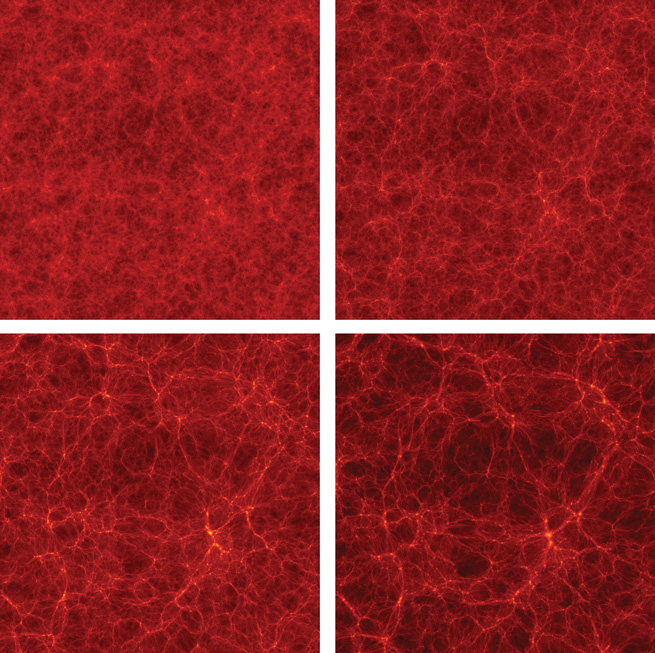
\includegraphics[width=0.85\textwidth]
	{./figures/3_nbody_simulations/Bolshoi_Evolution.png}

	\caption{\small{Evolución de la simulación Bolshoi. Se ilustran el
	campo de densidad de una región rectangular de 16 Mpc$/h$ de grosor y 
	250 Mpc$/h$	de lado para diferentes estadios de evolución. $z=9.5$ 
	(superior izquierda), $z=3$ (superior derecha), $z=1$ (inferior 
	izquierda) y $z=0$ (inferior derecha). Tomado de 
	\url{http://spectrum.ieee.org/aerospace/astrophysics/the-cosmological-supercomputer} }}
	
	\label{fig:Bolshoi_Evolution}
\end{figure}
%.........................................................................


Debido a su mayor tamaño comóvil comparada con las simulaciones 
restringidas (un cubo de $250$ Mpc$/h$ de lado), esta es usada para 
obtener estadística más fina en los resultados del capítulo 
\ref{cha:Results}. El modelo cosmológico usado para esta simulación 
corresponde al WMAP7 (ver tabla \ref{tab:CosmologicalParameters}), el número 
de partículas es de $2048^3$, lo que implica una masa promedio por partícula 
de $1.4 \times 10^8 h^{-1}$ M$_{\odot}$. Una descripción técnica más 
detallada de la simulación puede ser consultada en \cite{klypin2011}.


	%---------------------------------------------------------------------
	%Constrained simulations (CLUES)
	\subsection{Simulaciones Restringidas (CLUES)}
	\label{subsec:ConstrainedSimulations}
	%---------------------------------------------------------------------


Simulaciones restringidas

%.........................................................................
%Constrained Simulation
\begin{figure}[htbp]
	\centering
	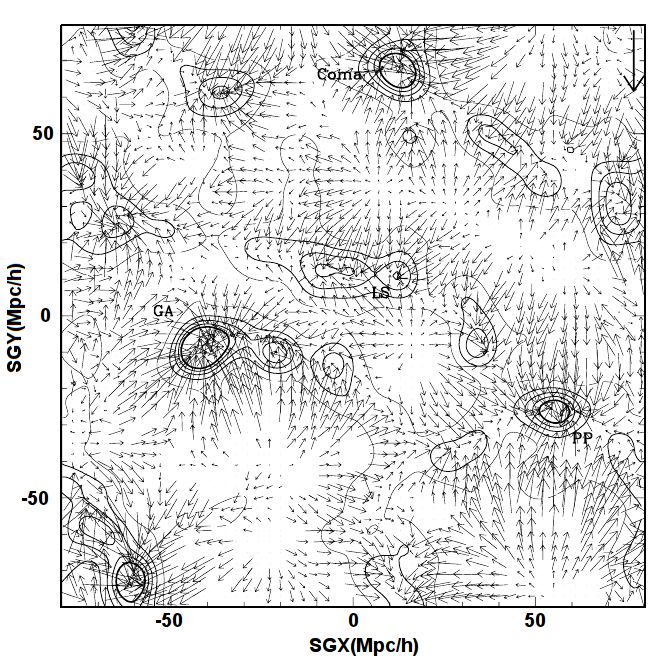
\includegraphics[width=0.8\textwidth]
	{./figures/3_nbody_simulations/Constrained_Construction.png}

	\caption{\small{Simulación Restringida}}
	
	\label{fig:Constrained_Construction}
\end{figure}
%.........................................................................
\newpage


%*************************************************************************



%*************************************************************************
%Environment Characterization
\section{Caracterización del Entorno}
\label{sec:EnvironmentCharacterization}


	%---------------------------------------------------------------------
	%The T-web Method
	\subsection{Método T-web}
	\label{subsec:TheT-webMethod}
	%---------------------------------------------------------------------


	%---------------------------------------------------------------------
	%The V-web Method
	\subsection{Método V-web}
	\label{subsec:TheV-webMethod}
	%---------------------------------------------------------------------


%*************************************************************************




%*************************************************************************
%Halos detection and sample definitions
\section{Detección de Halos y Definición de Muestras}
\label{sec:HalosDetectionAndSampleDefinitions}


	%---------------------------------------------------------------------
	%FOF method
	\subsection{Método FOF}
	\label{subsec:FOFMethod}
	%---------------------------------------------------------------------


	%---------------------------------------------------------------------
	%BDM method
	\subsection{Método BDM}
	\label{subsec:BDMMethod}
	%---------------------------------------------------------------------
	
	
	%---------------------------------------------------------------------
	%Sample of pairs to use
	\subsection{Muestra de Pares a Usar}
	\label{subsec:SampleOfPairsToUse}
	%---------------------------------------------------------------------
	
	
	%---------------------------------------------------------------------
	%Pair finder method
	\subsection{Método de Detección de Pares}
	\label{subsec:PairFinderMethod}
	%---------------------------------------------------------------------


%*************************************************************************




%.........................................................................
%Curved Spaces
\begin{figure}[htbp]
	\centering
	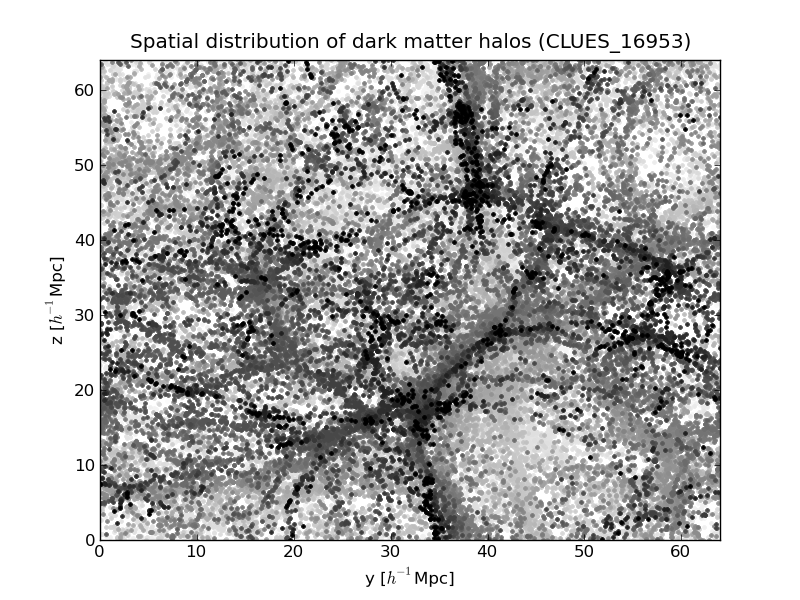
\includegraphics[width=0.49\textwidth]
	{./figures/3_nbody_simulations/Halos_Spatial_Distribution(CLUES_16953).png}
	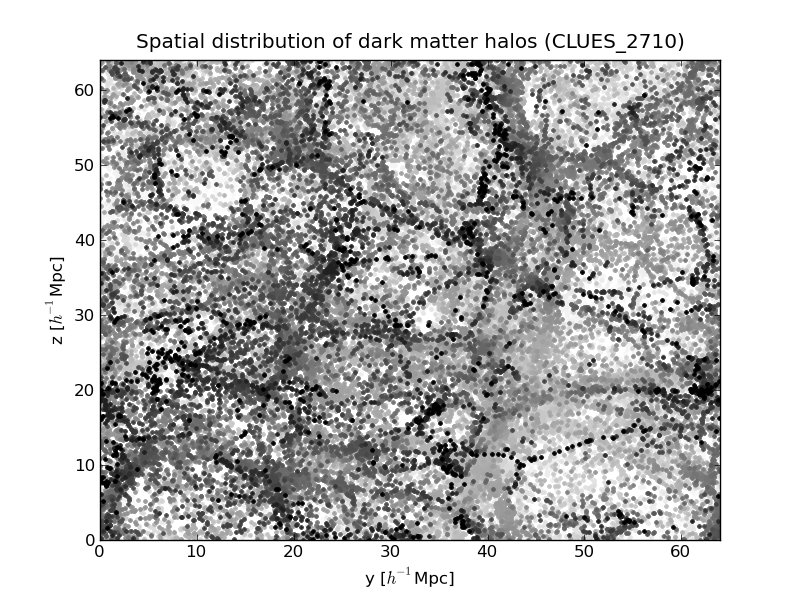
\includegraphics[width=0.49\textwidth]
	{./figures/3_nbody_simulations/Halos_Spatial_Distribution(CLUES_2710).png}
	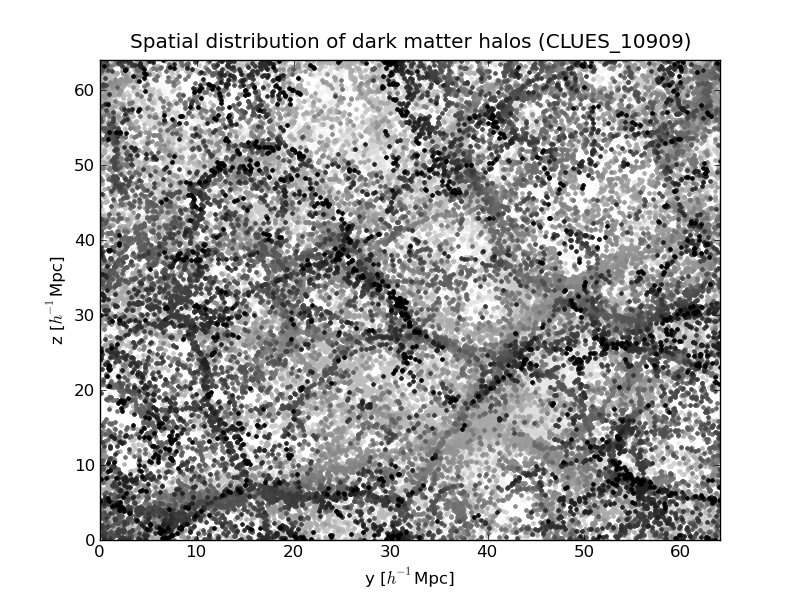
\includegraphics[width=0.49\textwidth]
	{./figures/3_nbody_simulations/Halos_Spatial_Distribution(CLUES_10909).png}

	\caption{\small{Halos en las simulaciones CLUES.}}
	
	\label{fig:CLUES}
\end{figure}
%.........................................................................